	

% We need layers to draw the block diagram
\pgfdeclarelayer{background}
\pgfdeclarelayer{foreground}
\pgfsetlayers{background,main,foreground}


\tikzstyle{frontEndPart} = [draw, fill=blue!20, text width=22em, text centered, minimum height=2.5em]
\tikzstyle{backEndBackground} = [draw, fill=green!10, text width=35em, minimum height=7em, rounded corners, dashed]
\tikzstyle{intermediatePart} = [draw, text width=10em, minimum height = 2em]
\tikzstyle{backEndPart} = [draw, fill=green!30, text width=10em, minimum height=2em]
\tikzstyle{execPart} = [draw, text width=9em, minimum height=2em, text centered]


\begin{figure}[b!]
\begin{center}

	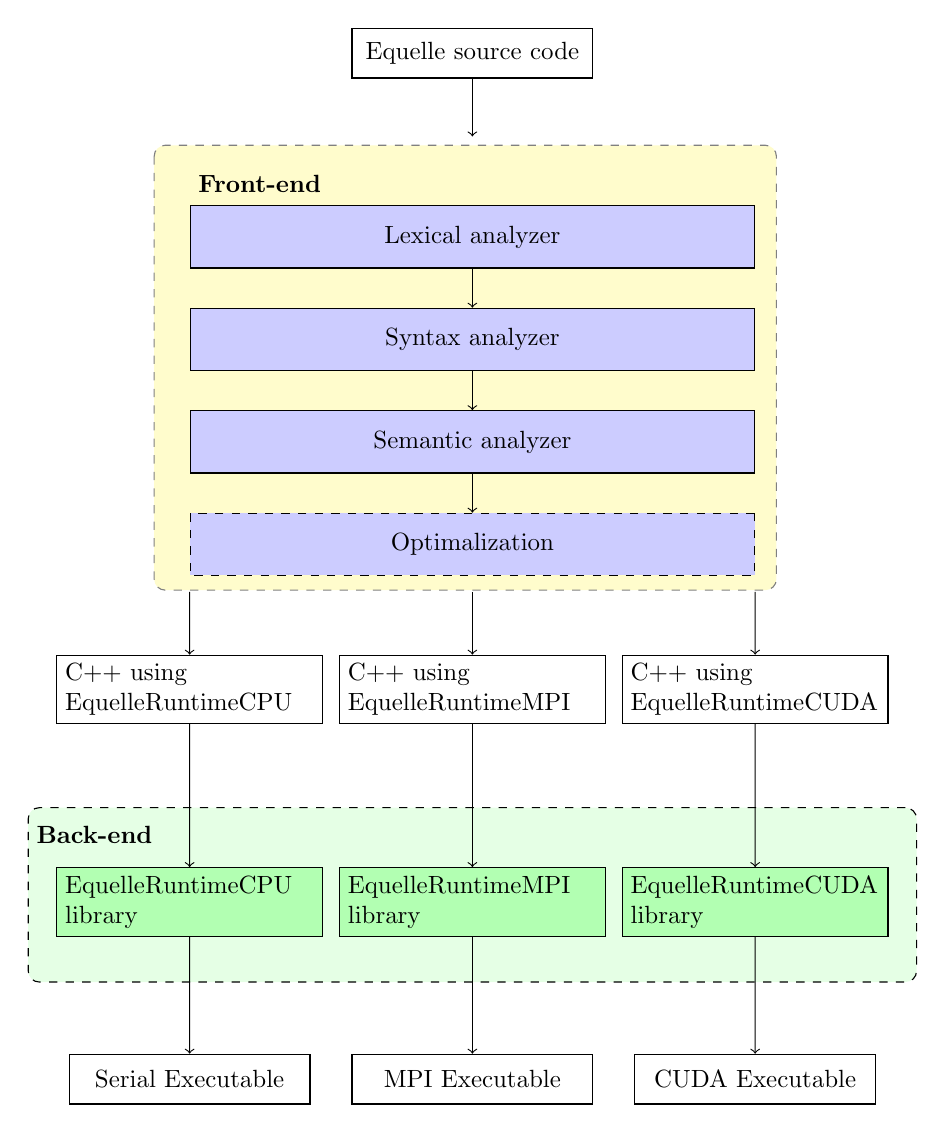
\begin{tikzpicture}[scale=0.9, transform shape]
		\node (frontendText) [text width=22em] {\textbf{Front-end}};
		\path (frontendText.-90)+(0,-0.5) node (lexical) [frontEndPart] {Lexical analyzer};
		\path (lexical.-90)+(0,-1) node (syntax) [frontEndPart] {Syntax analyzer};
		\path (syntax.-90)+(0,-1) node (semantic) [frontEndPart] {Semantic analyzer};
		\path (semantic.-90)+(0,-1) node (optimization) [frontEndPart, dashed] {Optimalization};
		
		\path [draw, ->] (lexical) -- (syntax);
		\path [draw, ->] (syntax) -- (semantic);
		\path [draw, ->] (semantic) -- (optimization);
		
		\begin{pgfonlayer}{background}
			 % Compute a few helper coordinates
        			\path (frontendText.west |- frontendText.north)+(-0.5,0.3) node (frontEndNorthWest) {};
        			\path (optimization.south -| optimization.east)+(+0.3,-0.2) node (frontEndSouthEast) {};
        			\path[fill=yellow!20,rounded corners, draw=black!50, dashed]
          		  (frontEndNorthWest) rectangle (frontEndSouthEast);
		\end{pgfonlayer}
		
		\path (frontendText.north)+(0,0.3) node (frontEndNorth) {};
		\path (frontEndNorth)+(0,1.3) node (sourceCode) [execPart] {Equelle source code};
		%\node (sourceCode) [above of=frontendText, node distance = 1.7cm] {Equelle source code};
		\path [draw, ->] (sourceCode) -- (frontEndNorth);
		
		% Helpers to locate arrows from front end
		\path (optimization.west |- optimization.south)+(0,-0.1) node (toSerial) {};
		\path (optimization.south)+(0,-0.1) node (toMPI) {};
		\path (optimization.east |- optimization.south)+(0,-0.1) node (toCUDA) {};
		
		\path (toSerial)+(0,-1.5) node (serial) [intermediatePart] { C++ using \\ EquelleRuntimeCPU};
		\path (toMPI)+(0,-1.5) node (mpi) [intermediatePart] { C++ using \\ EquelleRuntimeMPI};
		\path (toCUDA)+(0,-1.5) node (cuda) [intermediatePart] { C++ using \\EquelleRuntimeCUDA};
		
		\path [draw, ->] (toSerial) -- (serial);
		\path [draw, ->] (toMPI) -- (mpi);
		\path [draw, ->] (toCUDA) -- (cuda);
		
		\begin{pgfonlayer}{foreground}
			\path (serial)+(0,-3) node (serialBackend) [backEndPart] {EquelleRuntimeCPU library};
			\path (mpi)+(0,-3) node (mpiBackend) [backEndPart] {EquelleRuntimeMPI library};
			\path (cuda)+(0,-3) node (cudaBackend) [backEndPart] {EquelleRuntimeCUDA library};
			
			\path [draw, ->] (serial) -- (serialBackend);
			\path [draw, ->] (mpi) -- (mpiBackend);
			\path [draw, ->] (cuda) -- (cudaBackend);
		\end{pgfonlayer}
		
		\begin{pgfonlayer}{background}
			\path (optimization.-90)+(0,-4.5) node (backend) [backEndBackground] {\textbf{Back-end} \bigskip $\quad$ \bigskip $\quad$ \bigskip $\quad$ \bigskip $\quad$};
		\end{pgfonlayer}
	
		\path (serialBackend)+(0,-2.5) node (serialExec) [execPart] {Serial Executable};
		\path (mpiBackend)+(0,-2.5) node (mpiExec) [execPart] {MPI Executable};
		\path (cudaBackend)+(0,-2.5) node (cudaExec) [execPart] {CUDA Executable};
		
		\path [draw, ->] (serialBackend) -- (serialExec);
		\path [draw, ->] (mpiBackend) -- (mpiExec);
		\path [draw, ->] (cudaBackend) -- (cudaExec);

		
	\end{tikzpicture}
	\caption{The Equelle compiler}
	\label{fig:equelle:compiler}
\end{center}
\end{figure}


